44. \begin{figure}[ht!]
\center{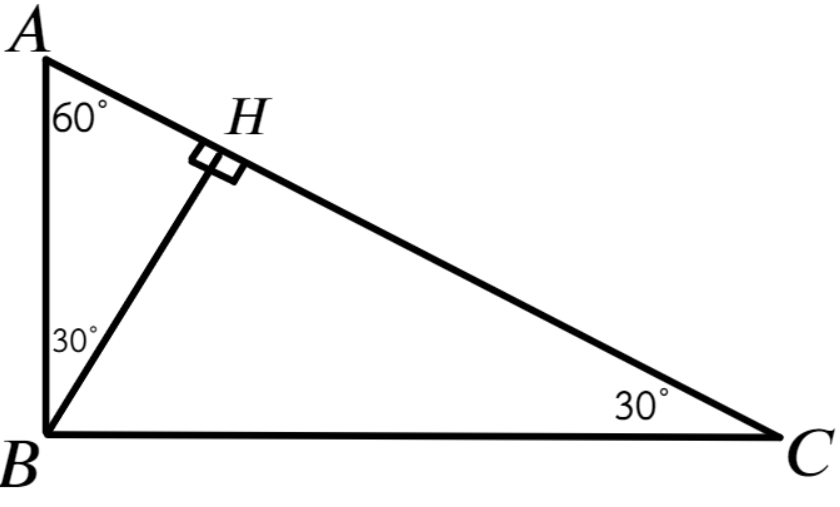
\includegraphics[scale=0.35]{g43.png}}
\end{figure}\\
Пусть $\angle C=30^\circ,$ тогда $\angle A=90^\circ-30^\circ=60^\circ,\ \angle ABH=90^\circ-60^\circ=30^\circ.$ По теореме о катете, лежащем напротив угла в $30^\circ,$ для треугольников $ABH$ и $ABC$ имеем $AB=2AH,\ AC=2AB=4AH.$ Значит, $AH=AC:4=6:4=1,5$см, а $HC=AC-AH=6-1,5=4,5$см.\\
